
\chapter{Introduction}

The Standard Model (SM) of particle physics continues to be one of mankind's 
greatest intellectual achievements.  It provides a mathematically elegant 
description of the building blocks of matter (quarks and leptons) and the 
forces through which they interact.  With the discovery of the Higgs boson at the
Large Hadron Collider in 2012 by both the ATLAS and CMS experiments
\cite{Aad:2012tfa, Chatrchyan:2012xdj}, all particles predicted by the SM have
now been observed.  However, there remain many outstanding issues which the SM
fails to explain.  

One such issue is the composition and nature of dark matter. The 
existence of dark matter was first inferred in the early 1930s by Zwicky when
calculating the velocity dispersion of the galaxies in the Coma cluster 
\cite{Zwicky:1933gu}.  Using the velocity dispersions, Zwicky calculated the 
cluster's mass using the virial theorem and found it to be $\sim$400 times 
larger than what was expected from their luminosity.  He then concluded that 
the Coma cluster contained far more of some yet unobserved \emph{dunkel Materie}
or `dark matter' than luminous matter.  Additional evidence would come 
a few decades later when Rubin and Ford observed that the rotational velocity
of galaxies was approximately flat instead of decreasing as $1/\sqrt{r}$ as 
expected \cite{Rubin:1980zd}.  More recent results based on gravitational
lensing \cite{Clowe:2006eq} and the cosmic microwave background 
\cite{Adam:2015rua}, further strengthen the argument for the existence of dark 
matter.

In 2008, the observation by the Payload for Antimatter Matter Exploration and 
Light-nuclei Astrophysics (PAMELA) of an unanticipated rise in the positron 
fraction \cite{Adriani:2008zr} sparked a surge of interest in so called 
``hidden sector'' models.  Some of these models suggest that dark matter 
inhabits a hidden sector with its interactions mediated by a massive 
photon-like particle \cite{ArkaniHamed:2008qn, Pospelov:2008jd, Hooper:2012cw}.
In fact, the possibility that nature contains an 
additional gauge boson  ($A'$, ``dark'', ``hidden'', ``heavy'' photon) was 
first considered by Holdom \cite{Holdom:1985ag}.  According to Holdom, 
an additional $U(1)$ gauge
symmetry of nature would ``kinetically mix'' with the SM photon, in turn, 
inducing an effective gauge coupling of the heavy photon to electric charge, 
which is suppressed by a factor of $\epsilon \sim 10^{-2} - 10^{-12}$.  
Kinetic mixing between the $A'$ and the SM photon establishes a portal through which
the properties of not only dark matter but other hidden sector particles can be
explored.

The effective coupling of the heavy photon to electric charge allows its 
production through a process analogous to bremsstrahlung radiation.  The Heavy
Photon Search (HPS)  is a fixed target experiment that utilizes this production
mechanism to search
for heavy photons in the mass range of 10 MeV/$c^2$ to 1 GeV/$c^2$.  Using 
Jefferson Lab's high luminosity electron beam along with a compact, large
acceptance forward spectrometer consisting of a silicon vertex tracker and a
lead tungstate electromagnetic calorimeter, HPS will access unexplored regions
in the mass-coupling phase space. The estimated reach of the HPS experiment at 
2$\sigma$ significance along with existing limits 
(see Section \ref{sec:current_limits}) are shown on Figure 
\ref{fig:ap_limits}. The reach calculation assumes running at 1.1
GeV (solid gold line) and 2.2 GeV (blue line) for a week each.  The full 
contour (dashed gold line) assumes an additional 2 weeks of 4.4 GeV running. 
Sensitivity to the upper region is achieved through a resonance search while
the lower region utilizes a resonance search plus a displaced vertex.
\begin{figure}[h!t]
    \centering
    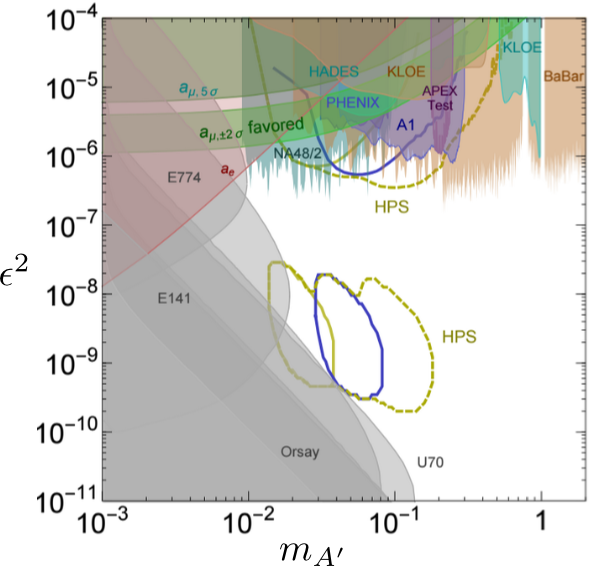
\includegraphics[width=0.80\textwidth]{images/ap_current_constraints.png}
    \caption{The estimated reach of the Heavy Photon Search experiment at 
             2$\sigma$ significance along with existing constraints from 
             beam dump  \cite{},
             collider \cite{}, 
             and fixed target experiments \cite{}.  The green band labeled 
             ``$a_{\mu} \pm 2\sigma$ favored'' represents the region that an 
             $A'$ can be used to explain the discrepancy between the measured 
             and calculated muon anomalous magnetic moment.  The regions 
             labeled ``$a_e$'' and ``$a_\mu$'' are exclusions based on the 
             anomalous magnetic moments of the muon and electron.
             The reach calculation assumes HPS running at 1.1 GeV 
             (solid gold line) and 2.2 GeV (blue line) for a week each.  The
             full contour (dashed gold line) assumes an additional 2 weeks of 
             4.4 GeV running.}
    \label{fig:ap_limits}
\end{figure}

This dissertation will present the results of a resonance search for a heavy 
photon in the mass range of 20 MeV/$c^2$ and 60 MeV/$c^2$ using the 2015 HPS
engineering run data set.  The search uses 74 nb$^{-1}$ of unblinded data which 
amounts to less than 10\% of the data collected during the engineering run.
An analysis using the full engineering run dataset will be completed in the 
summer of 2016. Chapters 2-3 will motivate the need to search for heavy 
photons and provide an overview of its production mechanism.  Chapters 4-5 
detail the HPS detector and its performance.  Finally, Chapter 6 will contain
the details of the resonance search along with results and discussion.
